\section{Virtual circuits at the FileDownload Agent Level}

\subsection{Changes to the FileDownload agent}

For this prototype we decided to integrate all of the control and circuit awareness
logic in the FileDownload agent, thus eliminating the need for an additional site 
agent or any changes to the DB schema. 

To ease development and to facilitate testing, we fake calls to circuit management APIs
which in turn, return IPs of already established static circuits. From PhEDEx'
point of view it's as if a new path has been created. If some conditions are
met, PhEDEx switches to using this path, as it would with a dynamic circuit.

\subsubsection{Making use of a circuit}

PhEDEx transfers files in bulk, copying several files with each transfer command. The number of files varies from
site to site depending on local constraints, but is typically in the range of a few tens of files per transfer job. Each transfer job therefore contains information about the source and destination Physical File Names (PFNs) of several files.

A PFN contains the protocol that needs to be used, the hostname or IP of the file
and the local path of that file. This means that if we want PhEDEx to use
circuits, we need a mechanism to replace the original hostname or IP in each 
source/destination PFN with the source IP and destination IP of the circuit.

The FileDownload agent actually receives only Logical File Names (LFNs) from the database, plus the name of the chosen source site. It constructs the PFNs from the LFNs and a lookup-table per-site which each site maintains and uploads to the database. After calculating the source and destination PFNs, files are bundled into transfer jobs and queued for submission with whichever transfer tool has been configured between the two sites.

When the transfer jobs are taken from the local queue, but before they are actually submitted, the agent will check to see if a circuit has been established between the two endpoints. If so, it manipulates the source and destination PFNs, replacing the hostnames or IP numbers of the endpoints with the IP numbers corresponding to the circuit. This manipulation is completely transparent to the actual transfer tool in use.

It could also happen that a circuit becomes available, while the FileDownload agent
marks tasks ready for transfer. This means that part of the tasks in a job
will contain source/destination PFNs having the original hostname/IPs, while
others will use the circuit IPs. When the FDT backend is used, it will automatically
launch two different jobs: one for the files transferred over the normal path
and the other for files transferred over the circuit. We still need to test
how the other backends react. In any case, even if a transfer job would fail 
because of this, PhEDEx will just retry, as it would for any failure, and the transfer would succeed the second
time.

\subsubsection{Circuit awareness and lifecycle management}

Since the standard FileDownload agent doesn't have knowledge about more than one
transfer paths over a given link we needed to add this circuit awareness and a
way to manage the lifecycle of a circuit on a given link.

PhEDEx agents are event-driven, using the Perl Object Environment (POE\cite{POE}) framework.
To implement circuit-control we added several POE controlled events. Here are the main ones:

\begin{itemize}
  \item check\_workload
  \item request\_circuit
  \item handle\_request
  \item teardown\_circuit
  \item check\_circuit\_setup
\end{itemize}

\paragraph{check\_workload}
This is a recurrent event at 60 second intervals. It is used to estimate the 
amount of work that remains to be done based on the current size of the download
 queue. In order to do this, it needs to know the average rate that the current 
link is capable of and the total number of pending bytes. The latter is calculated
based on the PENDING tasks that it currently holds. The former can be retrieved
in two ways: 

\begin{itemize}
  \item if the agent has recently transfered tasks it will retain information about
previously DONE tasks, which will then be used for the average rate calculation
  \item if nothing has been transferred, it will try to get this information based
on the link average rate calculated by PhEDEx itself.
\end{itemize}

If an average rate source-destination pair has been calculated, it will estimate
the amount of work needed to be done.

Going through all of the links, we check if all of the conditions below had been met:
\begin{itemize}
  \item the amount of work pending is above a given amount\footnote{This is arbitrarily set to five hours}
  \item a circuit has not been established
  \item a circuit request is not pending
  \item a circuit request hasn't failed within a given time-window\footnote{This time-window is arbitrarily set to one hour}
  \item transfers haven't previously failed, within a given time-window, while a circuit was active 
\end{itemize}

If this is the case, we trigger the request\_circuit event for that particular link.

\paragraph{request\_circuit}

As the name suggests this event is used to request a circuit.

It does the following:
\begin{itemize}
  \item creates a state-file for this request. This file contains the names of the PhEDEx nodes involved in the request, the time of the request and the 
lifetime of the circuit. This file is used to maintain knowledge of circuits across restarts of the FileDownload agent
  \item sets a timer to cancel the request if there is no timely response. If we don't
get a circuit within 10 minutes it's very likely that we won't get it at all.
  \item in the case of this prototype the "handle\_request" event is triggerred directly,
however in the production version, this event will actually be a callback
from the API call where a circuit is being requested
\end{itemize}

\paragraph{handle\_request}

This event is a callback from the API call to request a circuit.

It will:
\begin{itemize}
  \item trigger the event "remove\_circuit\_request"
  \item if the circuit creation failed, flag it and return
  \item modify and save the state file corresponding to this request by
adding relevant information concerning the circuit that has just been established:
time the circuit was established, time the circuit expires, endpoint IPs of 
the established circuit.
  \item starts a timer for the "teardown\_circuit" event if an expiration
time has been specified for the circuit
\end{itemize}

\paragraph{check\_circuit\_setup}

This is another recurrent event at 60 second intervals and is used to provide
sanitation in case of errors. There are two important scenarios that we are interested in:
\begin{enumerate}
  \item Download agent has crashed and is restarted
  \begin{enumerate}
    \item In-memory state information is lost, but circuit-request state file(s) exist on disk:\\
			For each circuit-request state file that has no matching in-memory data,
			try to cancel the circuit request and remove the file from disk
    \item In-memory state information is lost, but circuit-established state file(s) exist on disk:\\
			For each circuit-established state file that has no matching in-memory data,
			check the expiration time in the state file:
			\begin{itemize}
			  \item if the expiration time is not defined, or is defined but didn't expire yet,
					  the circuit can be reused. Internal data is populated based on state
					 file and if the expiration time is defined, the teardown\_circuit timer is
					 set.
			  \item if the expiration time is defined at it expired, remove the state file and
					 try to tear down the circuit 
			\end{itemize}
  \end{enumerate}
  \item Reconsider failed circuits with failed requests or transfers:\\
		  Creating a circuit on a particular link may have been blacklisted due to requests
		  for circuits failing or due to files transfers failing on that circuit. After a given
		  time these circuits are removed from the blacklist and the system is free to try
		  to use them again.
\end{enumerate}

\begin{description}
	\item[handle\_request\_timeout]
		Triggered after a timeout, cancels a request and cleans its internal state
	\item[remove\_circuit\_request]
		Cleans up internal data and state file concerning this circuit request
	\item[teardown\_circuit]
		Cleans up internal data and state file concerning the circuit and calls the API for 
		tearing down the circuit.
\end{description}

\subsection{Setup and test}

The prototype was tested on ANSE's testbed (Figure \ref{fig:ANSE-setup}) using 
our two PhEDEx sites: \\ T2\_ANSE\_Amsterdam and T2\_ANSE\_Geneva. As we mentioned earlier
each LSI controller manages 8 SSDs split in two RAID 0 arrays. Since the tests are write 
 intensive and were scheduled to run for around 24 hours, we decided to only use 
 1 LSI controller, in order to minimize the negative effects on the life of the SSDs.
Two 10Gbps virtual circuits were created for the purposes of this test. Figure \ref{fig:testbed}
depicts the setup used.

\begin{figure}[h]
  \centering
  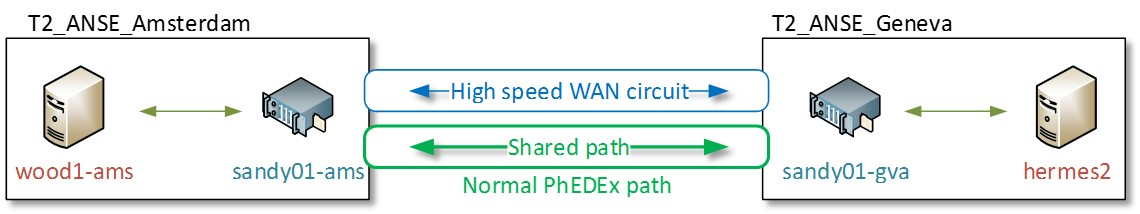
\includegraphics[width=0.95\textwidth]{Figures/FileDownload_ANSE_Testbed}
  \caption{Diagram of the testbed used by the prototype}
  \label{fig:testbed}
\end{figure} 

One of the circuits was used to model a shared link in which PhEDEx had to compete 
with other traffic. This background traffic was generated by Iperf and consisted of a 
continuous stream of UDP packets at 5Gbps . The other circuit served as the dedicated
link.

The main purpose of this test wasn't to show that we can saturate a 10Gbps link with
PhEDEX (although we came close with just 1 LSI controller), but that a PhEDEx FileDownload agent 
is able to switch to using a new path in a transparent manner and with no down time.

The first part of the test consisted of a 10 hour run with PhEDEx transfers on the 
shared link. After this time, PhEDEx switched to using the dedicated circuit and
continued transfers for another 10 hours. We set up PhEDEx to run a single 450 GB transfer 
job at a time, each one comprised of 30 files of 15 GB each.

\subsection{Results}

The results of the first half of the test are shown in  (Figure \ref{fig:shared_transfers}).
A quick glance at this plot, shows that the 10 Gbps link was saturated by the two
competing transfers. Between 23:00 and 0:00 (beginning of the plot) and 
10:00 and 11:00 (end of the plot), only UDP traffic was sent across the network, 
running at a steady 5 Gbps. This effectively leaves only 5 Gbps of PhEDEx traffic.
PhEDEx transfers start around 0:00 and quickly saturates the 10 Gbps. 
The seesaw look of this plot is due to the fact that PhEDEx has a delay
between finishing one job and starting the next. This is due to various factors:
 pre/post validation, preparation of copyjobs or even time spent by the backend itself 
 before actually launching a transfer. Because of these delays, the average 
 rates reported by PhEDEx will always be lower than the average rates of each
 individual transfer job. Nevertheless we get average transfer rates of 9.5 Gbps for the
 whole link and consequently 4.5 Gbps for PhEDEx transfers (10\% penalty from
 gap between jobs).

\begin{figure}[h]
  \centering
  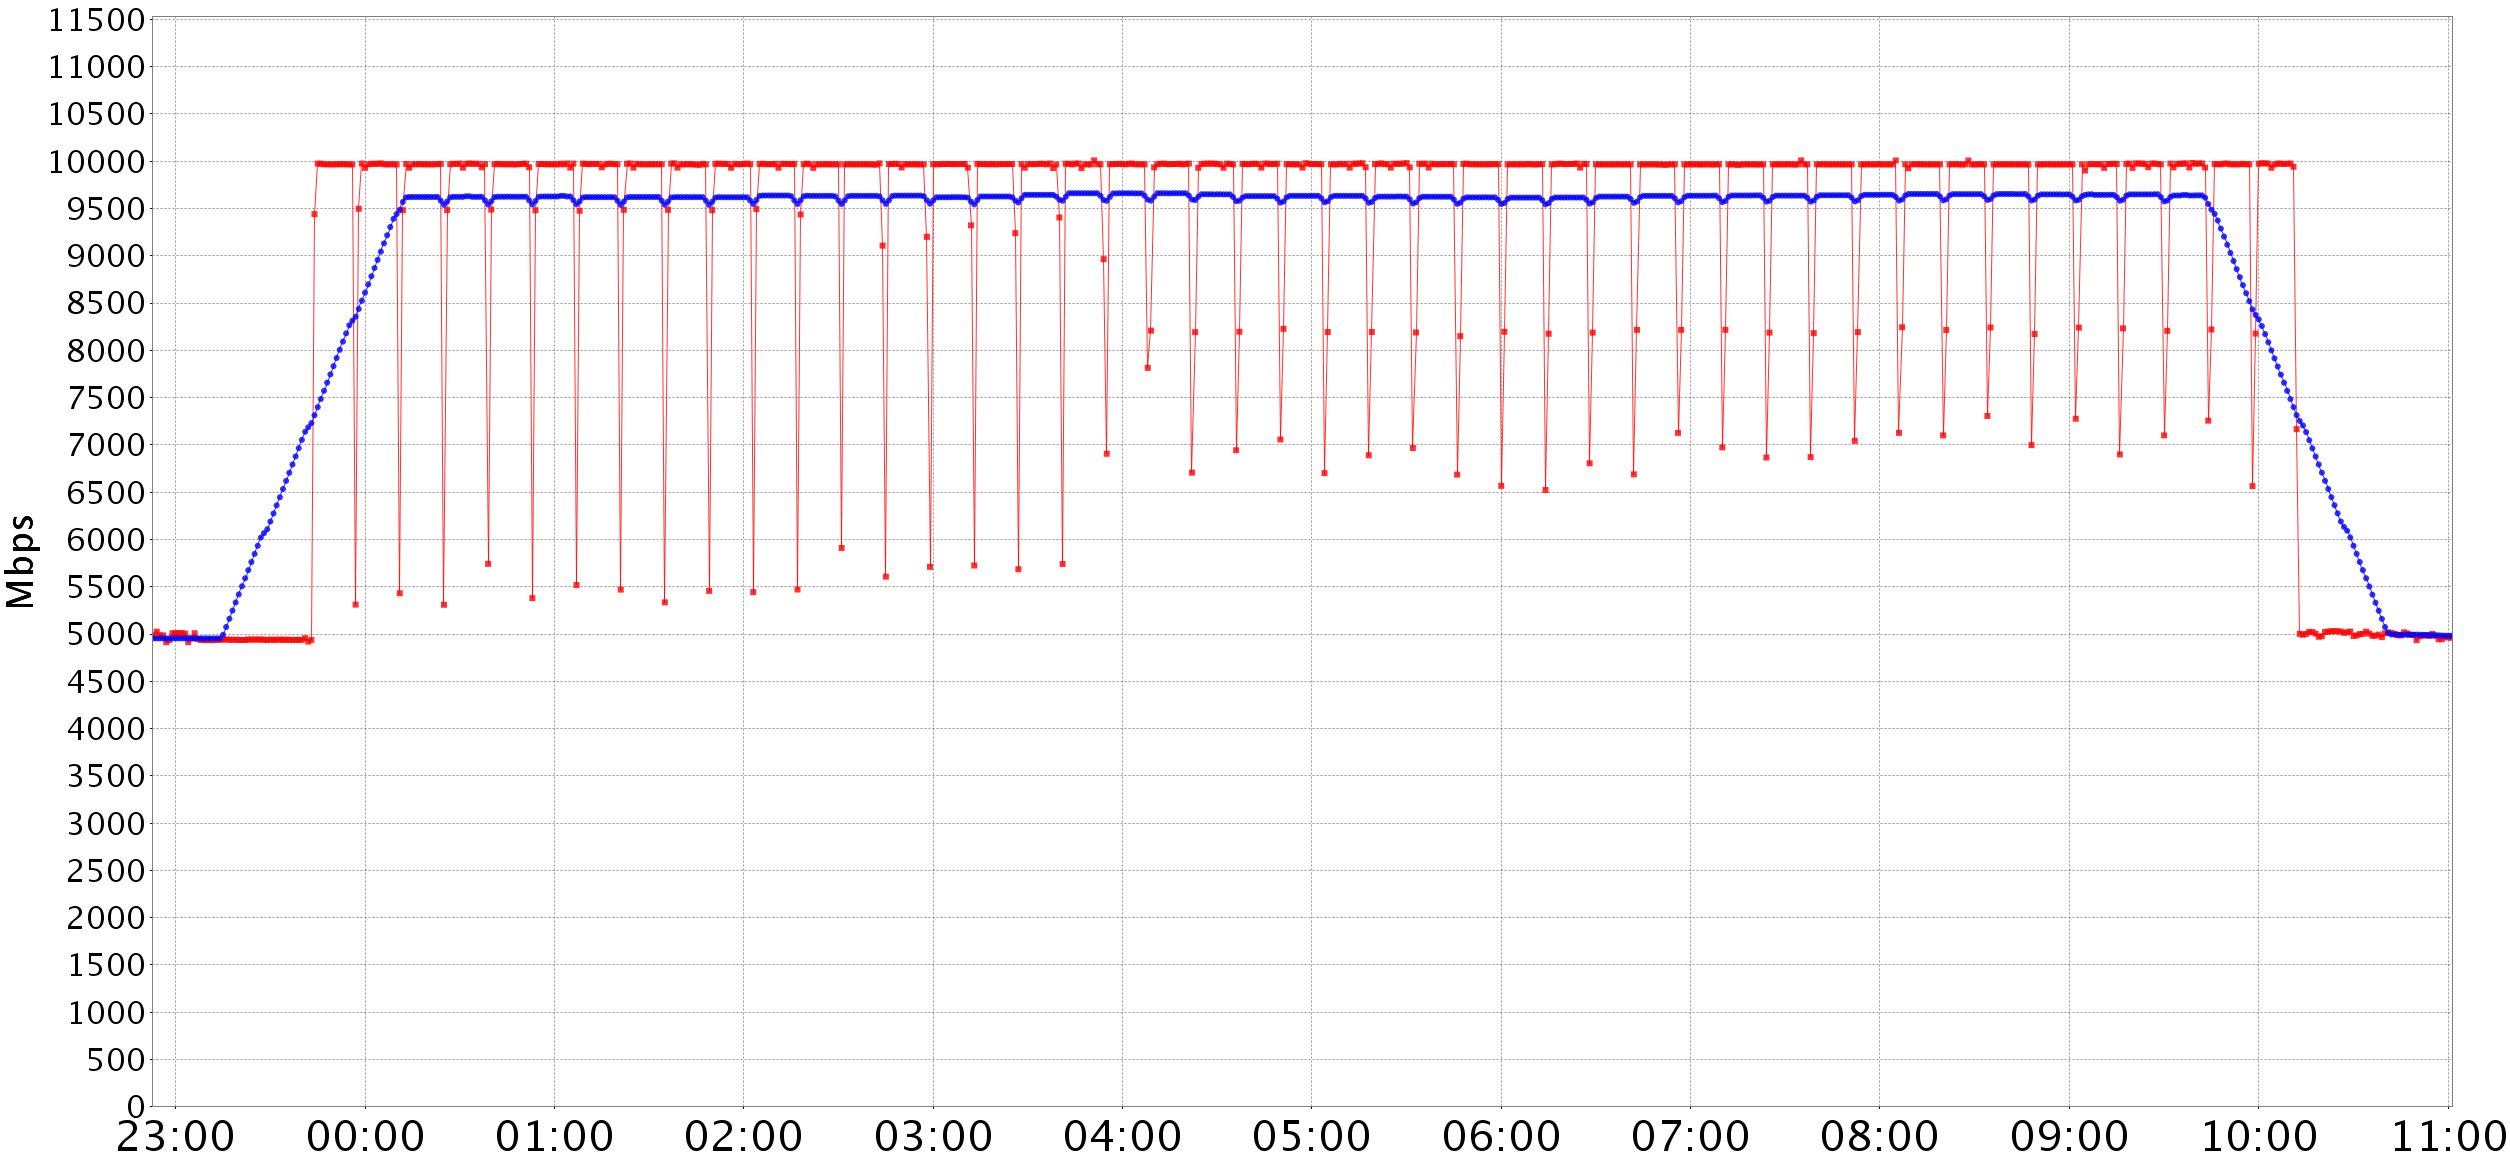
\includegraphics[width=0.95\textwidth]{Figures/FileDownload_Shared_path.png}
  \caption{PhEDEx transfers on the shared path - competing with 5Gbps UDP traffic. As with
  the previous case, the red line represents network throughput in Mbps while the blue
  line represents a moving average of one hours of that network throughput.}
  \label{fig:shared_transfers}
\end{figure} 

Around 10:00 PhEDEx switches to using the dedicated link. The results of the 
second half of the test are shown in Figure \ref{fig:solo_transfers}.

Although most of the time we are able to saturate the 10Gbps link with PhEDEx 
traffic alone we sometimes see dips in transfer rates. These dips can be attributed 
to the storage not being able to sustain such high write rates.

This time, the average link rates drop from 9.5 Gbps to 8.5 Gbps, however 
actual PhEDEx transfers go up from 4.5 Gbps to 8.5 Gbps! The reason for this 
drop in average link rate is two fold: 

\begin{itemize}
  \item Transferring a job at higher speeds means that it will take less time for
  it to complete, hence more jobs will be completed in one hour. However, as
  we previously explained, there is a fixed overhead for starting each new job, which
  means that more delays will be introduced into the system.
  \item The storage system (using 1 LSI controller) sometimes cannot sustain
  write rates of 10 Gbps to disk.
\end{itemize}

\begin{figure}[h]
  \centering
  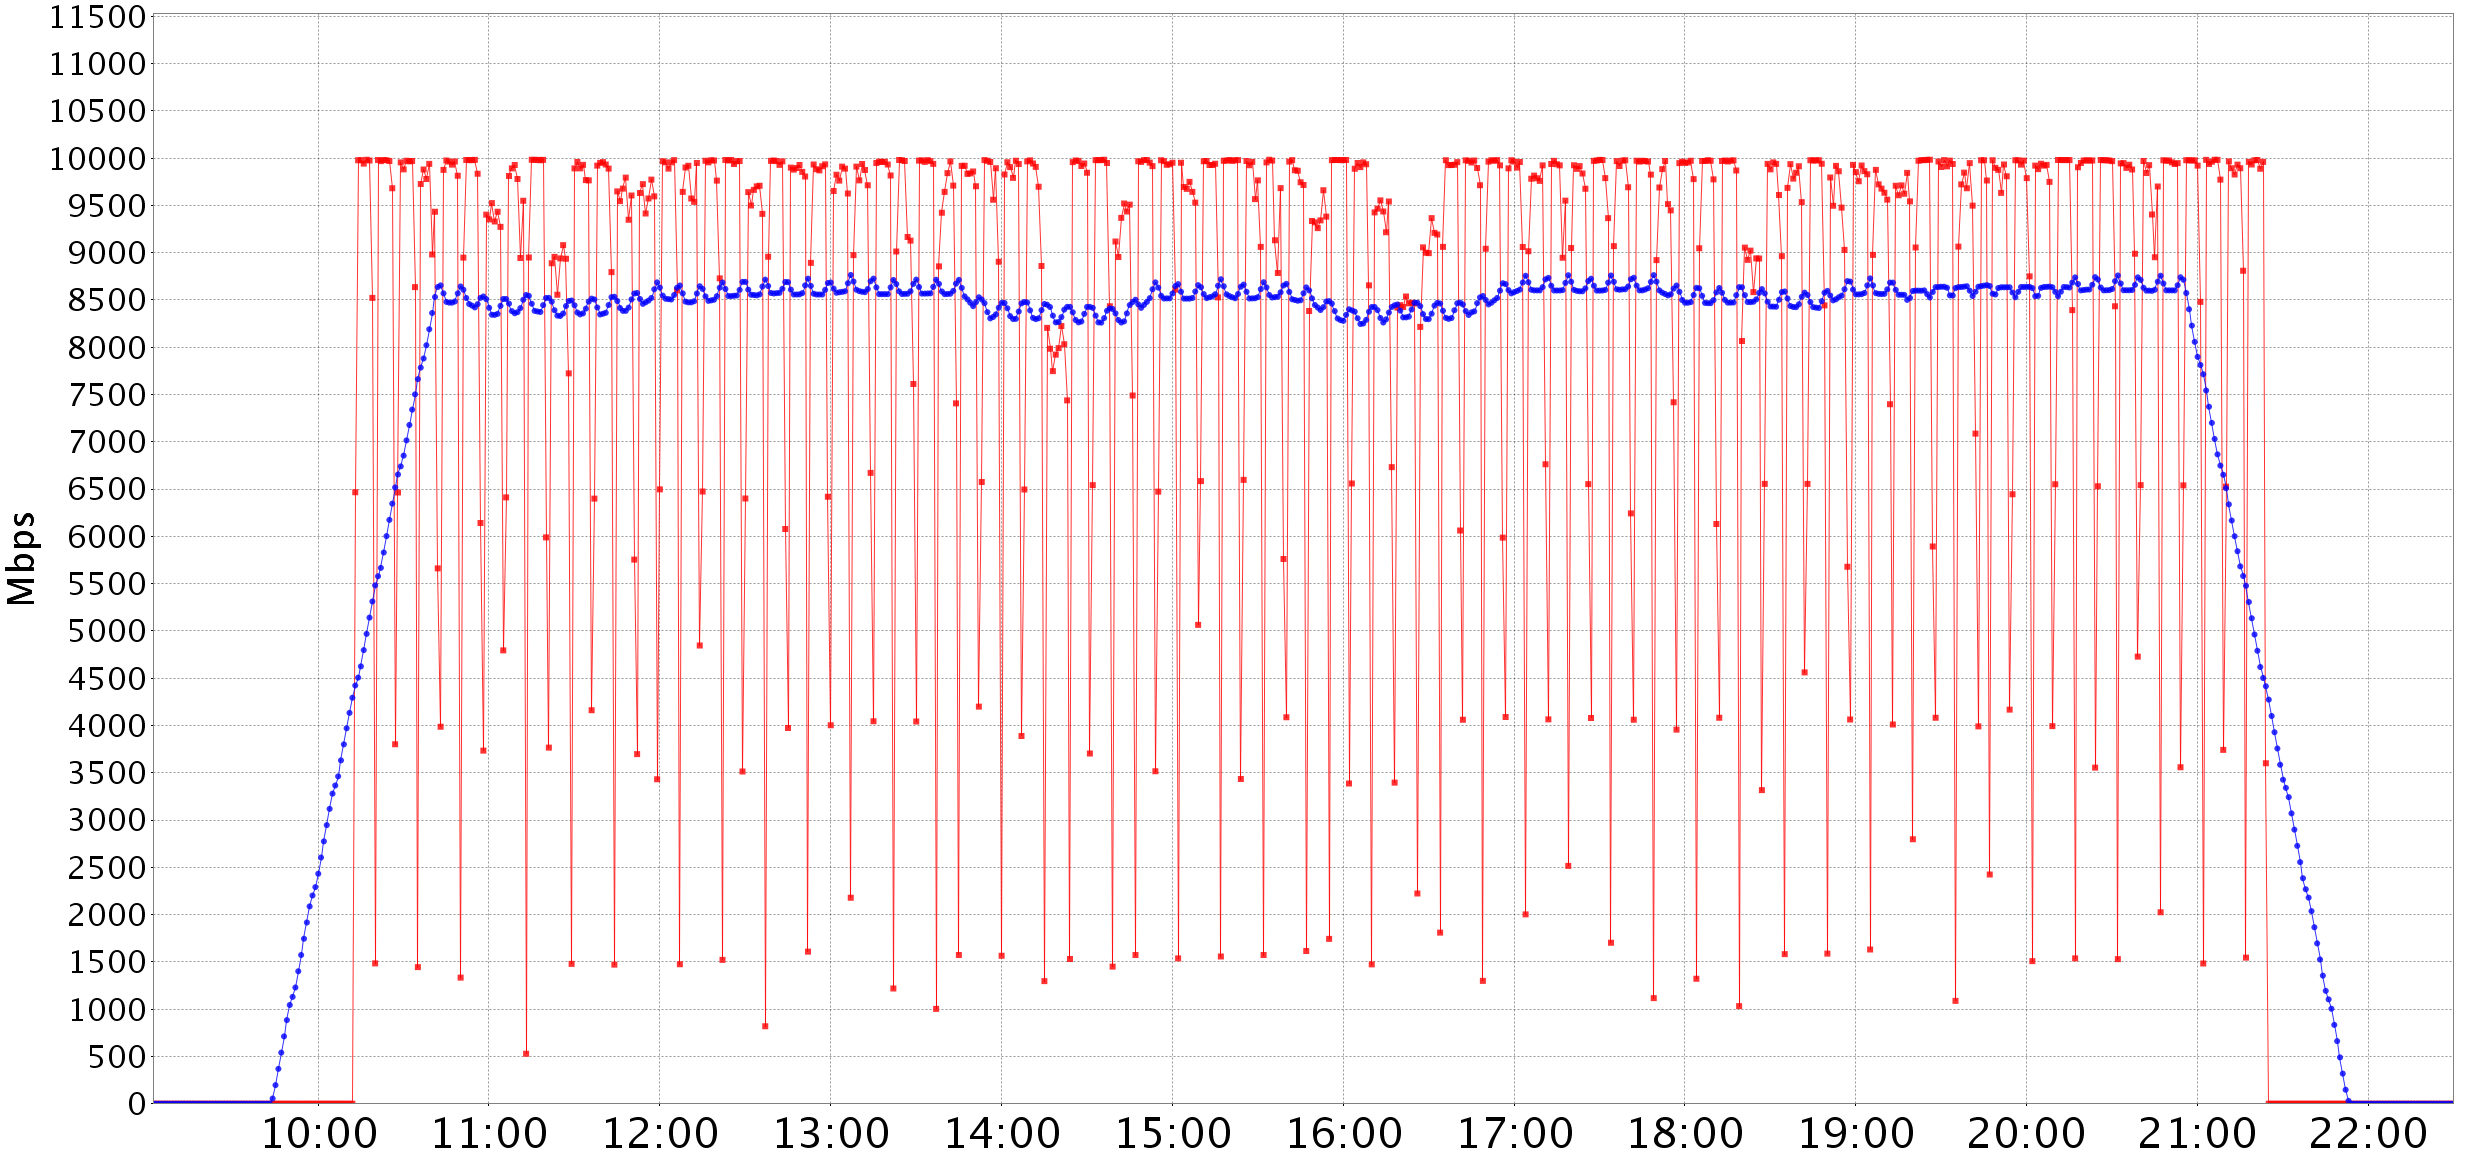
\includegraphics[width=0.95\textwidth]{Figures/FileDownload_Solo_path.png}
  \caption{PhEDEx transfers on the dedicated path}
    \label{fig:solo_transfers}
\end{figure} 

Figure \ref{fig:combined_transfers} and Figure \ref{fig:combined_phedex_transfers} show
the  network activity for PhEDEx traffic alone on both links. 
In this plot we can observe that PhEDEx switches to using the
new link without any interruption in service, doing it seamlessly and in a 
transparent way for other site-agents (switch occurs around 10:00).

\begin{figure}[h]
  \centering
  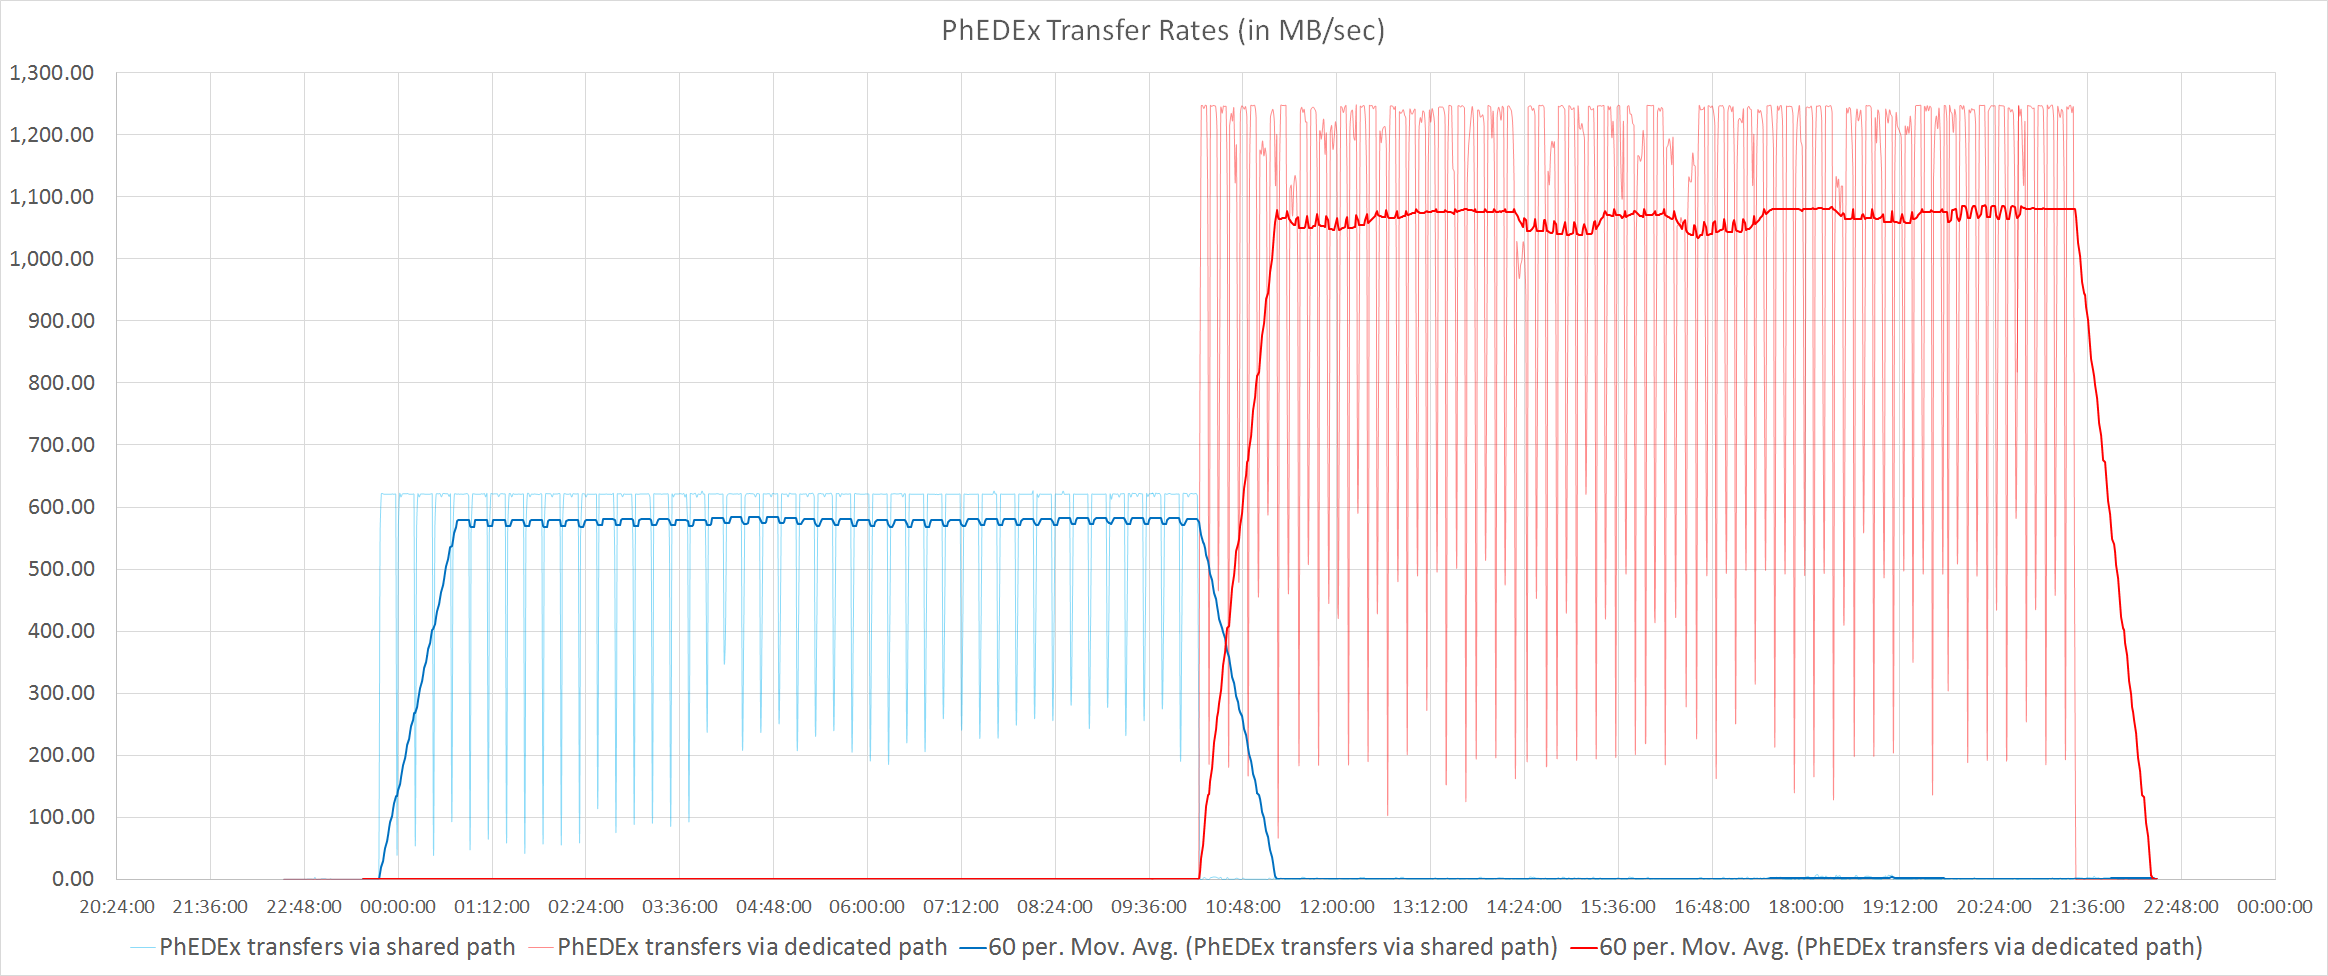
\includegraphics[width=0.95\textwidth]{Figures/FileDownload_All_paths.png}
  \caption{View of PhEDEx-only transfers on both the shared and dedicated path}
  \label{fig:combined_transfers}
\end{figure} 

\begin{figure}[h]
  \centering
  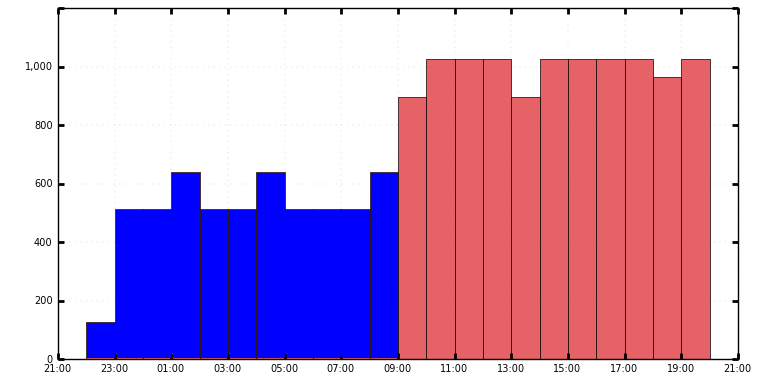
\includegraphics[width=0.95\textwidth]{Figures/FileDownload_PhEDEx_all_paths.png}
  \caption{View of PhEDEx only transfers on both the shared and dedicated path}
  \label{fig:combined_phedex_transfers}
\end{figure} 